\labsection{Введение}

Как известно, вещество может находиться в трёх фазовых состояниях~--- твёрдом, жидком и газообразном, причём эти
состояния последовательно сменяются по мере возрастания температуры. Если~и дальше нагревать газ, то сначала молекулы распадаются на атомы, а~затем и атомы распадаются на электроны и ионы, так что газ становится ионизованным, представляя собой смесь из свободных электронов и ионов, а~также нейтральных частиц. Если \important{степень ионизации} газа, под которой принято понимать отношение числа ионизованных атомов к их полному числу, достаточно велика, то такой сильно ионизованный газ может обладать качественно новыми свойствами по сравнению с обычным газом. Прежде всего такой газ обладает высокой электропроводностью и поэтому, в противоположность нейтральному газу, сильно взаимодействует с электрическим и магнитным полями. Кроме того, заряженные частицы в таком газе стремятся распределиться в пространстве таким образом, чтобы установилась локальная квазинейтральность, то есть равенство концентраций положительных и отрицательных частиц, нарушаемое тепловыми флуктуациями только в микроскопических масштабах. Такое состояние ионизованного газа называется \important{плазмой.}  Более точное определение этого понятия будет дано далее. Плазму называют также четвёртым состоянием вещества.


Первое описание газовой плазмы дал И.~Ленгмюр (1923~г.), исследуя электрический разряд в газе низкого давления (тлеющий разряд). Он назвал плазмой <<ярко светящийся газ, состоящий из электронов, ионов разных сортов и нейтральных атомов и молекул>>. Он же ввёл сам термин~--- плазма (от греческого глагола, обозначающего <<разрыхляться>>, <<расползаться>>)~--- и основные параметры, характеризующие плазму: плотности составляющих её частиц~--- электронов~--- $n_e$, ионов~--- $n_i$,нейтральных частиц~--- $n_0$ и их температуры~--- соответственно $T_e$, $T_i$,~$T_0$.

Очевидно, что свечение плазмы, являющееся следствием непрерывно идущей рекомбинации электронов и ионов в нейтральные атомы, сопровождается выделением энергии и уменьшением концентрации электронов и ионов. Стационарное состояние плазмы, которое мы только и будем исследовать, может существовать лишь при наличии непрерывно действующего источника ионизации. Им может быть электрический разряд в газе (газоразрядная плазма), происходящий в постоянном электрическом поле (обычный газовый разряд, дуга и т.~д.) или в высокочастотном поле (индукционные катушки, запитанные током высокой частоты электроды и т.~д.). Плазма может образовываться и при термической ионизации газа, если газовая среда поддерживается при достаточно высокой температуре (звёзды, пламя газовой горелки). Плазма образуется в фокальной области мощных лазерных установок и при многих других условиях.

Степень ионизации плазмы обычно невелика. В тлеющем газовом разряде (люминесцентные лампы) плотность электронов
составляет примерно $10^9~\text{см}^{-3}$, а плотность нейтральных молекул ${\sim}10^{14}~\text{см}^{-3}$. Лишь внутри звёзд и в
специальных установках, используемых для исследования проблем, связанных с управляемым термоядерным синтезом,
относительное число атомов, находящихся в ионизированном состоянии, приближается к единице (полностью ионизованная
плазма). Мощность, подводимая к таким установкам, измеряется мегаваттами.

Плазма исследуется также в связи с проблемой создания магнитогидродинамических генераторов~--- преобразователей
механической энергии движущегося в магнитном поле проводящего газа в электрическую энергию.

Ещё одно важное направление использования плазмы~--- применение её для проведения химических реакций, которые в горячей
сильно ионизованной газовой среде происходят очень быстро и эффективно.

Температура плазмы, как правило, измеряется не в градусах, а в эле-ктрон-вольтах ($1~\text{эВ}\approx 11\,600~\text{К}$). При расчётах
плазменных явлений обычно используется система СГС.

Стационарное (не меняющееся со временем) состояние плазмы может быть равновесным или неравновесным. В первом случае
компоненты плазмы (электроны и ионы) имеют одну и ту же температуру, а во втором~--- разную. При достаточно больших
давлениях (звёзды, пламя газовой горелки) между компонентами плазмы может успевать установиться тепловое равновесие. При
малых давлениях ($\lambda\ge d$, где $\lambda$~--- длина свободного пробега, а $d$~--- характерный размер занятой
плазмой области) тепловое равновесие устанавливаться не успевает. Так, в тлеющем газовом разряде мы обычно имеем дело с
<<горячими>> электронами и <<холодными>> ионами. Электроны быстро ускоряются электрическим полем и почти не теряют
энергии при соударении с тяжёлыми ионами и атомами газа, а также при столкновении со стенками газоразрядной трубки.
Наоборот, ионы быстро отдают полученную от поля энергию нейтральным атомам газа и атомам стенок, поскольку массы их
близки. В результате реализуются условия, при которых электроны характеризуются одной~--- более высокой, а ионы~---
другой, более низкой температурой.

Большой интерес представляет плазма, существующая в атмосфере Земли и планет, а также в космосе. Атмосферная плазма
создаётся ультрафиолетовым излучением Солнца. Электроны плазмы захватываются магнитным полем Земли (движутся вокруг и
вдоль силовых линий магнитного поля) и образуют радиационные пояса на расстояниях тысяч километров от поверхности Земли.
Широко известны также плазменные проводящие слои Хевисайда, обеспечивающие дальнюю радиосвязь на коротких волнах.


\begin{figure}[h!]
	\psfrag{x}[br]{\footnotesize $n$, см\^{-3}}
	\psfrag{y}{\footnotesize $T$, эВ}
	\psfrag{a}[cr]{\footnotesize $10^{-2}$}
	\psfrag{b}[cr]{\footnotesize $10^{-1}$}
	\psfrag{c}[cr]{\footnotesize $1$}
	\psfrag{d}[cr]{\footnotesize $10$}
	\psfrag{e}[cr]{\footnotesize $10^{2}$}
	\psfrag{f}[cr]{\footnotesize $10^{3}$}
	\psfrag{g}[cr]{\footnotesize $10^{4}$}
	\psfrag{h}[cr]{\footnotesize $10^{5}$}
	\psfrag{A}[ct]{\footnotesize $1$}
	\psfrag{B}[ct]{\footnotesize $10^{10}$}
	\psfrag{C}[ct]{\footnotesize $10^{20}$}
	\psfrag{D}[ct]{\footnotesize $10^{30}$}
	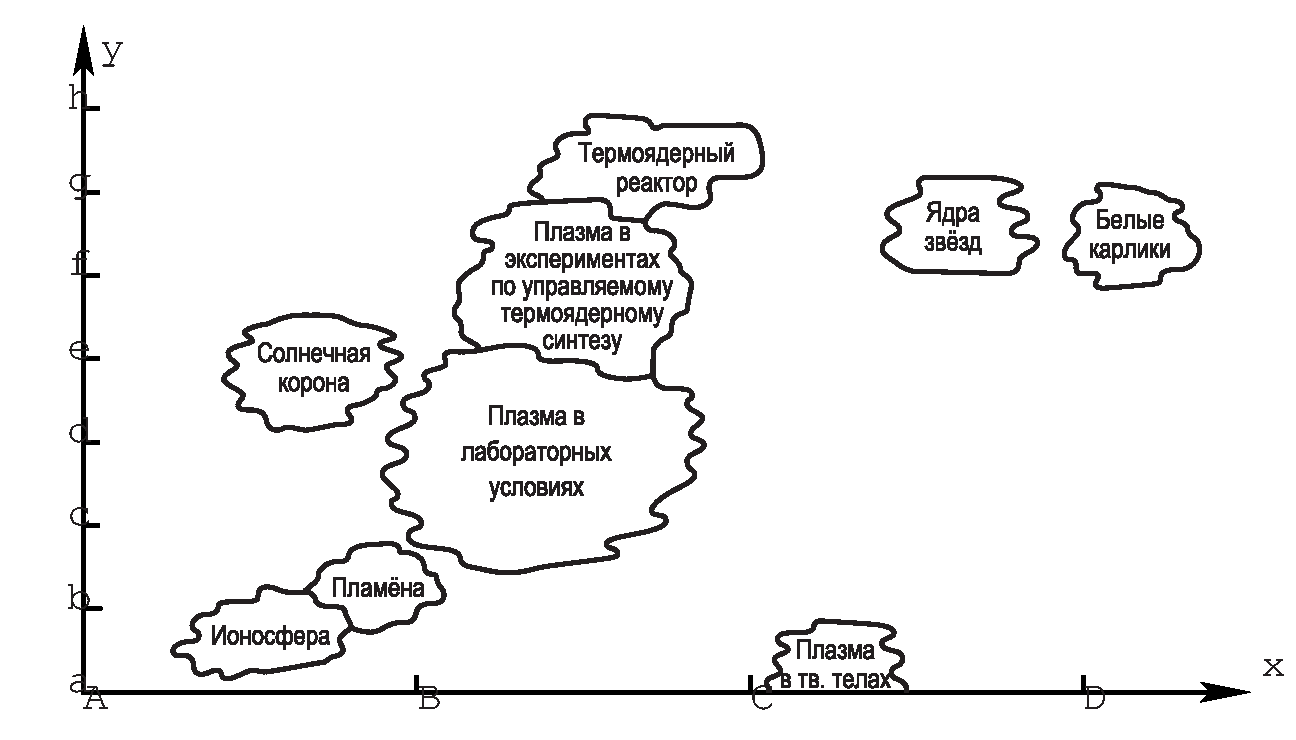
\includegraphics[width=0.9\textwidth]{Chapter_5/v5_0}
	\caption{Различные типы плазмы в лаборатории и природе}
	\figmark{Types of plasma}
\end{figure}

Свойствами, характерными для газовой плазмы, обладают и некоторые другие среды, называемые по этой причине
плазмоподобными средами, или просто плазмами: в этом смысле термин \important{плазма} встречается в научной литературе во множественном числе.
\todo[author = Andrew]{В картинке для нанесения некоторых обозначений был использован psfrag, который несовместим с pdf. Необходимо исправить изображение.}
В качестве примеров различных плазм можно назвать плазму металлов, электронно-дырочную плазму
полупроводников, нуклонную плазму атомного ядра и т.~д. Различные типы плазм, встречающихся как в лабораторных условиях,
так и в природе, можно достаточно наглядно представить на плоскости параметров: температура плазмы~--- плотность числа
частиц (рис.~\figref{Types of plasma}). Под температурой плазмы в каждом конкретном случае понимают температуру тех заряженных частиц, которые
определяют плазменные свойства рассматриваемой среды: в большинстве случаев это электроны.

\labsection{Некоторые свойства плазмы}

Как уже говорилось выше, определяющим свойством плазмы является её квазинейтральность. Это означает, что во всяком
сколько-нибудь большом объёме заряды ионов и электронов всегда компенсируют или почти компенсируют друг друга. Если хотя
бы на некоторое время это оказывается не так, то возникают сильные электрические поля, которые перемещают электроны и
ионы и восстанавливают квазинейтральность плазмы.

Оценим размер области, внутри которой могут существовать заметные электрические поля. Рассмотрим пространство вокруг
иона, имеющего положительный заряд и поэтому притягивающего электроны, поле которых противоположно по знаку полю иона.
Ион <<экранируется>> электронами, так что его поле убывает с увеличением расстояния $r$ не по закону $1/r^2$, а
существенно сильнее. Если бы не тепловое движение электронов, то они так <<облепили>> бы ион, что его поле было бы
полностью скомпенсировано (точнее, произошла бы рекомбинация). Тепловое движение мешает такой компенсации. Рассчитаем
этот эффект.

Как известно, электрическое поле $E$ и плотность электрического заряда $\rho$ в однородной среде связаны между собой
уравнением
\begin{equation}
	\eqmark{5.1}
	\Div \vec{E}=4\pi\rho.
\end{equation}

Переходя от напряжённости поля $\vec{E}$ к электрическому потенциалу $\varphi$ с помощью обычного соотношения
\begin{equation}
	\eqmark{5.2}
	\vec{E}=-\Grad\varphi,
\end{equation}
получим уравнение Пуассона:
\begin{equation}
	\eqmark{5.3}
	\Delta\varphi=-4\pi\rho,
\end{equation}
где $\Delta$~--- оператор Лапласа. Поле заряда сферически симметрично, поэтому в сферической системе координат оно зависит только от радиуса. Оператор Лапласа в этом случае принимает простую форму:
\begin{equation*}
	\Delta=\frac{d^2}{dr^2}+\frac{2}{r}\frac{d}{dr},
\end{equation*}
поэтому уравнение Пуассона принимает вид:
\begin{equation}
	\eqmark{5.4}
	\frac{d^2\varphi}{dr^2}+\frac{2}{r}\frac{d\varphi}{dr}=-4\pi\rho.
\end{equation}

В силу большой инерционности ионов ($m_i~\gg~m_e$) по сравнению с электронами далее мы будем считать ионы вообще бесконечно
тяжёлыми, то есть неподвижными, что, как показывают точные расчёты, не меняет ответа по порядку величины.

Распределение электронов, а значит, и плотность их пространственного заряда $\rho_e$ подчиняется формуле Больцмана:
\begin{equation}
	\eqmark{5.5}
	\rho_e=-ne\cdot e^{e\varphi/kT_e}.
\end{equation}
где $k$ - постоянная Больцмана.

При написании \eqref{5.5} считалось, что плотность электронов на достаточном удалении от заряда (при $\varphi=0$) равна $n$.
Числом $e$ обозначена абсолютная величина заряда электрона, так что его заряд равен $-e$.

В соответствии со сделанным выше предположением ионы неподвижны. Их плотность пространственного заряда $\rho_i$ всюду одинакова и
равна своему значению в области $\varphi=0$, где она равна и противоположна по  знаку плотности пространственного заряда электронов.
Таким образом,
\begin{equation}
	\eqmark{5.6}
	\rho_i=ne ,
\end{equation}
то есть плазма вдали от источника кулоновского поля квазинейтральна. 

Подставляя \eqref{5.5} и \eqref{5.6} в \eqref{5.4}, получим:
\begin{equation}
	\eqmark{5.7}
	\frac{d^2\varphi}{dr^2}+\frac{2}{r}\frac{d\varphi}{dr}=-4\pi ne\left[1-e^{e\varphi/kT_e}\right].
\end{equation}

Это уравнение нелинейно и в аналитическом виде не решается. Решение может быть найдено, если считать, что:
\begin{equation}
	\eqmark{5.8}
	\frac{e\varphi}{kT_e}\ll1.
\end{equation}

В этом случае экспоненту можно разложить в ряд и уравнение \eqref{5.7} становится линейным:
\begin{equation}
	\eqmark{5.9}
	\frac{d^2\varphi}{dr^2}+\frac{2}{r}\frac{d\varphi}{dr}=\frac{1}{r_D^2}\varphi,
\end{equation}
где введено обозначение
\begin{equation}
	\eqmark{5.10}
	r_D=\sqrt{\frac{kT_e}{4\pi ne^2}}=743\sqrt{\frac{T_e~(\text{эВ})}{n~(\text{см}^{-3})}}~(\text{см}).
\end{equation}

Нетрудно убедиться путём подстановки, что решение уравнения \eqref{5.9} имеет вид
\begin{equation}
	\eqmark{5.11}
	\varphi=\frac{Ze}{r}e^{-r/r_D}.
\end{equation}

Это решение правильно ведёт себя около иона (где $\varphi\sim Ze/r$) и обращается в нуль на бесконечности. Мы нашли,
следовательно, искомое решение задачи. Оно показывает, что вследствие экранирующего действия электронов поле иона
убывает с расстоянием экспоненциально с характерной длиной, равной $r_D$~--- \important{дебаевскому радиусу экранирования (радиус Дебая, дебаевская длина).} Дебай ввёл понятие радиуса экранирования, рассматривая поле иона в
электролите.

Плазму можно считать почти нейтральной (квазинейтральной) в областях, размеры которых существенно превосходят дебаевскую
длину. При $T=10^4$~К ($\approx 1$~эВ) и $n=10^9 ~\text{см}^{-3}$, $r_D\approx 1,6\cdot10^{-2}$~см.

Теперь можно дать количественное определение понятия плазма.

\important{Плазмой} называется ионизованный газ, дебаевский радиус которого $r_D$ существенно меньше характерного
размера $l$ объёма, занимаемого этим газом, то есть
\begin{equation*}
	\sqrt{\frac{kT_e}{4\pi ne^2}}\ll l.
\end{equation*}

Это определение также принадлежит Ленгмюру.

Ещё одним важным параметром плазмы является число заряженных частиц (в среднем) в дебаевской сфере (сфера с радиусом,
равным $r_D$). Применённый при выводе дебаевского радиуса статистический подход (распределение Больцмана) предполагает,
что частиц должно быть много. Число частиц $N_D$ в дебаевской сфере можно оценить с помощью формулы \eqref{5.10},
подставляя в неё вместо истинного среднее число частиц (эти величины мало различаются):
\begin{equation}
	\eqmark{5.12}
	N_D\approx n\frac43\pi r_D^3\approx0,1\frac{(kT_e)^{3/2}}{n^{1/2}e^3}.
\end{equation}
Для плазмы газового разряда это число оказывается порядка $10^4$, т.~е. очень велико.

Заметим, что требование, чтобы число частиц в дебаевской сфере было велико по сравнению с единицей, эквивалентно
условию, что потенциальная энергия взаимодействия двух заряженных частиц в плазме существенно меньше их тепловой
энергии, то есть что плазма является газом, причём идеальным.

Другой важнейшей характеристикой плазмы является \important{плазменная} или \important{ленгмюровская} частота, выражение для
которой и её смысл можно получить из следующих соображений. Выделим в плазме объём в виде параллелепипеда, изображённого на рис.~\figref{1}. 

\begin{figure}[h!]
	\psfrag{E}[cb]{$E$}
	\psfrag{0}[ct]{0}
	\psfrag{X}{$X$}
	\psfrag{x}[ct]{$x$}
	\centering
	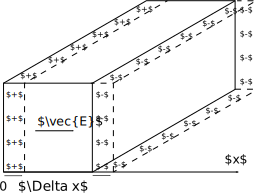
\includegraphics[width=0.3\textwidth]{Chapter_5/v5_1}
	\caption{???}
	\figmark{1}
\end{figure}

Сместим все электроны на расстояние $x$ относительно ионов (ионы занимают объём, изображённый сплошными, а
электроны~--- пунктирными линиями).
\todo[author = Andrew]{В картинке для нанесения некоторых обозначений был использован psfrag, который несовместим с pdf. Также отсутствует подпись к картинке. Необходимо исправить изображение.}
Пусть плотность электронов (и ионов) равна $n$; ионы для простоты будем считать
однозарядными. Легко видеть, что в результате такого смещения на гранях параллелепипеда возникнут поверхностные заряды:
\begin{equation}
	\eqmark{5.13}
	\sigma=nex.
\end{equation}

Вследствие этого появится электрическое поле:
\begin{equation}
	\eqmark{5.14}
	E=4\pi\sigma=4\pi nex.
\end{equation}

Это поле действует на электроны, придавая им ускорение, равное
\begin{equation}
	\eqmark{5.15}
	\frac{d^2x}{dt^2}=-\frac{eE}{m}=-\frac{4\pi ne^2}{m}x.
\end{equation}

Уравнение \eqref{5.15} определяет плазменную (ленгмюровскую) частоту коллективных колебаний электронов:
\begin{equation}
	\eqmark{5.16}
	\omega_p=\sqrt{\frac{4\pi n e^2}{m_e}}=5,65\cdot10^4\sqrt{n~(\text{см}^{-3})}.
\end{equation}

Плазменная частота задает естественный масштаб времени для плазмы: это~--- время отклика на флуктуацию плотности заряда в
плазме. Учитывая это, дебаевский радиус экранирования можно интерпретировать следующим образом. Пусть какая-то группа
электронов получила направленную скорость, равную тепловой: $v=\sqrt{kT_e/m_e}$. При этом, как легко можно убедиться,
обращаясь к формулам \eqref{5.16}, \eqref{5.10}, за время, равное $\omega_p^{-1}$, эта группа электронов пройдёт в направлении
полученной скорости до полной остановки расстояние, как раз равное дебаевской длине, то есть
\begin{equation}
	\eqmark{5.17}
	r_D=\frac{v}{\omega_p}.
\end{equation}

Таким образом, дебаевская длина~--- это амплитуда ленгмюровских колебаний плазмы, возбуждаемых тепловыми флуктуациями.
Эта амплитуда и является масштабом нарушения квазинейтральности плазмы в отсутствие внешнего поля.

Как следует из \eqref{5.16}, плазменная частота определяется только плотностью электронов (и универсальными постоянными).
Можно строго доказать, что она не зависит от формы рассматриваемого возмущения и является, таким образом,
локальной характеристикой плазмы. Плазменная частота является не единственной~--- но важнейшей~--- характерной частотой
плазмы. Она определяет коллективное движение электронов относительно ионов.

В заключение этого пункта сделаем следующее замечание. Формула для дебаевского радиуса \eqref{5.10} не учитывает движение
ионов. Если считать, что ионы тоже распределяются в поле пробного заряда по Больцману с температурой $T_i$, то в
приближении $e\varphi\le kT_i$, вместо формулы \eqref{5.10} получим
\begin{equation}
	\eqmark{5.18}
	r_D=\sqrt{\frac{k}{4\pi ne^2}\frac{T_eT_i}{T_e+T_i}},
\end{equation}
то есть вместо $T_e$ в формулу для дебаевского радиуса войдёт приведённая температура. В частности, при $T_e=T_i$ в
знаменателе под корнем появляется двойка, а при $T_e\gg T_i$, что имеет место для плазмы газового разряда (тлеющего), в
формуле \eqref{5.10} вместо $T_e$ будет стоять~$T_i$.

\labsection{Электропроводность плазмы}

Приложим к плазме электрическое поле с напряжённостью $\vec{E}$. Под его действием приходят в движение как электроны, так и
ионы. Действующие на них силы мало отличаются друг от друга, а массы различаются очень сильно. Основными носителями тока
являются поэтому электроны. Свободно двигаясь на пути свободного пробега, электроны приобретают направленную (дрейфовую)
скорость. После очередного соударения скорость электрона может иметь самые разные направления, так что среднее значение
этой скорости в начале пробега близко к нулю. В конце пробега оно равно
\begin{equation*}
	\vec{v}_\text{кон}=-\frac{e\lambda}{m_e\average{v_e}}\vec{E},
\end{equation*}
где $\lambda$~--- длина свободного пробега, а $\average{v_e}$~--- тепловая скорость электрона, по сравнению с
которой дрейфовая скорость обычно мала. Среднее значение дрейфовой скорости равно поэтому половине $v_\text{кон}$:
\begin{equation}
	\eqmark{5.19}
	v_\text{др}=\frac{e\lambda E}{2m_e\average{v_e}}.
\end{equation}

Средняя тепловая скорость $\average{v_e}$ определяется из обычной формулы:
\begin{equation}
	\eqmark{5.20}
	\average{v_e}=\sqrt{\frac{8kT_e}{\pi m_e}}.
\end{equation}

Объединяя эти формулы, найдём
\begin{equation}
	\eqmark{5.21}
	\vec{v}_\text{др}=-b\vec{E},
\end{equation}
где подвижность электронов $b$ равна
\begin{equation}
 	\eqmark{5.22}
	b=\frac{e\lambda}{2\sqrt{\frac{8m_e}{\pi} kT_e}}.
\end{equation}

Электропроводность плазмы $\sigma$ определяется совместным дрейфовым движением всех электронов, так что
\begin{equation}
	\eqmark{5.23}
	\sigma=\frac{j}{E}=\frac{n_eev_{др}}{E}=neb=\frac{e^2\lambda n_e}{2\sqrt{\frac{8m_e}{\pi} kT_ei}}.
\end{equation}

Полученная формула показывает, что электропроводность плазмы пропорциональна концентрации электронов и уменьшается с
ростом температуры плазмы. Длина свободного пробега $\lambda$ в слабоионизированной плазме определяется не столько
плотностью электронов $n_e$, сколько плотностью газа.

\labsection{Одиночный зонд}

Распределение электрического потенциала в плазме обычно определяют с помощью зондов~--- небольших проводников, вводимых в
плазму. Как уже говорилось выше, метод зондов был разработан Ленгмюром в начале двадцатых годов XX века.

Рассмотрим явления, происходящие при внесении в плазму уединённого проводника~--- зонда. Пусть электрический потенциал
зонда вначале равен потенциалу той точки плазмы, в которую будет помещён зонд. Поступающие на зонд токи электронов и
ионов в этом случае равны
\begin{equation}
	\eqmark{5.24}
	I_{e0}=\frac{n\average{v_e}}{4}eS,
\end{equation}

\begin{equation}
	\eqmark{5.25}
	I_{i0}=\frac{n\average{v_i}}{4}eS,
\end{equation}
\begin{wrapfigure}{o}{0.5\textwidth}
	\psfrag{x}{$X$}
	\psfrag{r}[tc]{$r_D$}
	\psfrag{f}[rb]{$\varphi(x)$}
	\psfrag{v}[cc]{$U_f$}
	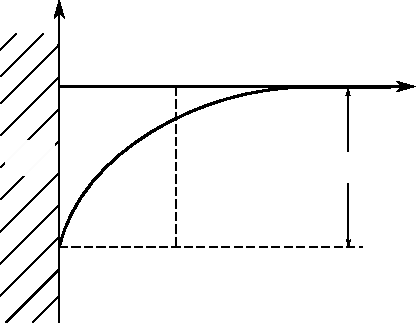
\includegraphics[width=0.5\textwidth]{Chapter_5/v5_8}
	\caption{Распределение потенциала в~окрестности зонда}
	\figmark{Potential distribution}
\end{wrapfigure}
\todo[author = Andrew]{В картинке для нанесения некоторых обозначений был использован psfrag, который несовместим с pdf. Необходимо исправить изображение.}
где $\average{v_e}$ и $\average{v_i}$~--- средние скорости электронов и ионов, $S$~--- площадь зонда, $n$~--- плотность
электронов и ионов (которые в силу квазинейтральности плазмы равны или почти равны друг другу). Множитель $\frac{1}{4}
n\average{v}$, согласно кинетической теории, определяет число ударов в секунду о единицу поверхности. Так как скорости
электронов существенно превосходят скорости ионов, то $I_{e0}\gg I_{i0}$, так что зонд заряжается до некоторого
отрицательного равновесного или, как обычно говорят, \important{плавающего} потенциала~$-U_f$. При плавающем потенциале
количество попадающих на зонд ионов и электронов уравнивается, так как до него могут доходить лишь наиболее быстрые
электроны и практически все ионы. Зонд, таким образом, приобретает отрицательный заряд. Вокруг него образуется область
положительного пространственного заряда (её ширина по порядку величины равна дебаевскому радиусу), экранирующего плазму
от зонда (рис.~\figref{Potential distribution}).

При установлении равновесия ионный ток мало меняется и в первом приближении по-прежнему определяется формулой
\eqref{5.25}\footnote{Как мы увидим ниже, эта формула при $U\approx -U_f$ на самом деле нуждается в поправках.}, а
выражение для электронного тока приобретает вид

\begin{equation}
	\eqmark{5.26}
	I_e=I_0\exp\left(-\frac{eU_f}{kT_e}\right),
\end{equation}
которое для плоских электродов следует из распределения Больцмана.

Возникновение <<дебаевского слоя>> вокруг зонда вносит некоторую неоп-ределённость в величину $S$: становится неясно,
какая площадь должна подставляться в формулы~--- площадь зонда или площадь поверхности этого слоя. При больших зондах
указанное различие несущественно, а при малых может оказаться важным.

Оценим величину плавающего потенциала. При равновесии электронный и ионный токи равны друг другу:
\begin{equation*}
	\frac{1}{4}n\average{v_i}eS=\frac{1}{4}n\average{v_e}eS\cdot\exp\left(-\frac{eU_f}{kT_e}\right),
\end{equation*}
откуда
\begin{equation}
	\eqmark{5.27}
	eU_f=kT_e\ln\frac{\average{v_e}}{\average{v_i}}=\frac12kT_e\ln\frac{T_em_i}{T_im_e}.
\end{equation}

В тлеющем газовом разряде $kT_e\approx 1$~эВ, а $kT_i\approx \frac{1}{40}$~эВ (комнатная температура). Положим для оценки
$m_i=10^4m_e$. Тогда
\begin{equation}
	\eqmark{5.28}
	eU_f%=\frac12\cdot 1~эВ\ln(40\.10^4)=
	\approx 6,5~\text{эВ}.
\end{equation}

Формулу \eqref{5.27} нельзя считать надёжной. При её выводе было сделано плохо оправданное предположение, что движение
ионов близко к тепловому. Это справедливо вдали от дебаевского слоя, но не около него и тем более не в нём, так как при
приближении к зонду дрейфовая скорость ионов быстро начинает превышать тепловую. Формула для величины ионного тока при
этом должна быть изменена. Тем не менее для грубых оценок она может быть использована.

Рис.~\figref{Potential distribution} иллюстрирует картину распределения потенциала вокруг зонда.

\labsection{Исследование плазмы с~помощью одиночных~зондов}

При исследовании плазмы с помощью зондов на них подаются напряжения и исследуются вольт-амперные
характеристики (ВАХ). Схема опытов изображена на \figref{Plasma study with single probe}, на котором изображены два погружённых в плазму электрода и
источник $\mathscr{E}$, создающий между ними регулируемую разность потенциалов. Пусть контактирующая с плазмой поверхность одного
электрода существенно меньше, чем у другого. Электрод с малой поверхностью будем называть зондом, а электрод с большой
поверхностью~--- опорным электродом. Рассмотрим, как зависит ток $I_з$ в цепи зонда от потенциала зонда~$U_з$
относительно опорного электрода.

\begin{figure}[h!]
	\centering
	\psfrag{I}[cc]{$I$}
	\psfrag{U}[cc]{$U$}
	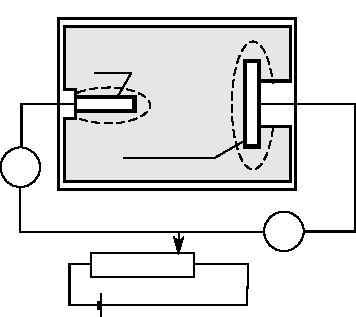
\includegraphics[width=0.7\textwidth]{Chapter_5/v5_9}
	\caption{К исследованию плазмы с~помощью одиночного~зонда}
	\figmark{Plasma study with single probe}
\end{figure}

Рассмотрим вначале случай, когда плазма эквипотенциальна. Пусть движок потенциометра (рис.~\figref{Plasma study with single probe}) установлен так, что зонд и
опорный электрод соединены накоротко. Ясно, что в этом случае они представляют собой один электрод сложной формы,
внесённый в плазму.
\todo[author = Andrew]{В картинке для нанесения некоторых обозначений был использован psfrag, который несовместим с pdf. Необходимо исправить изображение.}
Зарядившись отрицательно, они принимают относительно плазмы потенциал, равный плавающему потенциалу,
т.~е. $-U_f$. Полный ток на каждый электрод равен нулю, значит, электронный ток равен ионному.

Если плазма не эквипотенциальна, то ток зонда обращается в нуль лишь в том случае, если потенциалы зонда и опорного
электрода смещены на величину $U_f$ относительно потенциалов соответствующих участков плазмы. Необходимая для этого
разность потенциалов между зондом и опорным электродом равна разности потенциалов между соответствующими участками
плазмы. Измеряя потенциал зонда относительно опорного электрода (при нулевом токе), можно исследовать распределение
потенциала в плазме.

Сведения о температуре и плотности зарядов в плазме получают, снимая вольт-амперную характеристику зонда. Начнём
перемещать движок потенциометра (рис.~\figref{Plasma study with single probe}), т.~е. подавать на зонд некоторый потенциал. Через плазму и по внешней цепи
начинает проходить ток, так как баланс между электронным и ионным током нарушается. При этом
токи, проходящие через зонд и опорный электрод, конечно, равны друг другу, а плотности тока различны, так как площади
электродов существенно различаются. Плотность тока, идущего через опорный электрод, из-за большой площади последнего
всегда очень мала, и, следовательно, его потенциал относительно плазмы практически всегда равен $-U_f$. При небольшом
размере зонда наибольшая плотность тока возникает около него, так что практически всё падение напряжения приходится на
дебаевский слой, окружающий зонд.

Зависимость зондового тока $I_\text{з}$ от величины $U_\text{з}$ имеет вид, показанный на рис.~\figref{Single probe VAC} (мы снова рассматриваем
эквипотенциальную плазму). Эта кривая носит название зондовой характеристики. При $U_\text{з}<0$ весь ионный ток, приходящий на
границу дебаевского слоя, достигает зонда. Ионный ток равен, следовательно, своему максимальному значению, или, как
говорят, ионному току насыщения $I_{i\text{н}}$. 

\todo[author = Andrew]{В картинке для нанесения некоторых обозначений был использован psfrag, который несовместим с pdf. Необходимо исправить изображение.}
\begin{wrapfigure}{o}{0.5\textwidth}
	\psfrag{U}{$U_з$}
	\psfrag{I}[br]{$I_з$}
	\psfrag{0}[br]{0}
	\psfrag{a}[cr]{$I_{eн}-I_{iн}$}
	\psfrag{b}[cr]{$I_{eн}$}
	\psfrag{c}[cl]{$-I_{iн}$}
	\psfrag{d}[tc]{$U_f$}
	\psfrag{A}[rb]{$A$}
	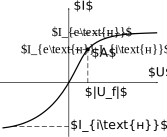
\includegraphics[width=0.5\textwidth]{Chapter_5/v5_10}
	\caption{Вольт-амперная характеристика одиночного~зонда}
	\figmark{Single probe VAC}
\end{wrapfigure}

При увеличении (по абсолютной величине) потенциала зонда электронный ток
уменьшается и, наконец, прекращается. Весь ток зонда является в этом случае ионным током. На первый взгляд, величина
тока при этом не должна зависеть от потенциала зонда. На самом деле это не так, поскольку при изменении потенциала
изменяется площадь поверхности дебаевского слоя и изменяются скорости ионов, которые быстро увеличиваются при
перемещении из плазмы к электроду~--- от тепловых значений до значений, определяемых величиной потенциала. Поэтому с
увеличением потенциала зонда (при смещении движка потенциометра влево на рис.~\figref{Plasma study with single probe}) ток зонда возрастает, хотя и не очень
сильно.

На правой ветви характеристики (при $U_\text{з}>0$) потенциал зонда превышает потенциал опорного электрода, но вначале (вплоть
до точки $A$) остаётся ниже потенциала плазмы. При этом ионный ток на зонд не меняется (вернее, слабо меняется), а
электронный ток возрастает. В точке $A$, т.~е. при $U_\text{з}=U_f$, слой пространственного заряда (дебаевский слой) исчезает и
оба тока~--- электронный и ионный~--- подходят к зонду беспрепятственно. При этом электронный ток, конечно, существенно
превосходит ионный, поскольку плотности электронов и ионов близки друг к другу, а тепловые скорости существенно
различаются.

При дальнейшем увеличении $U_з$ ионный ток подавляется, а ток электронов не изменяется и остаётся равным тепловому (на
самом деле, медленно возрастает по тем же причинам, по которым изменяется ионный ток насыщения).

Участок характеристики, расположенный влево от точки $A$, носит название \important{ионной} ветви (ионный ток равен току
насыщения), а участок вправо от точки $A$ называется \important{электронной} ветвью вольт-амперной характеристики
(электронный ток равен току насыщения).

Оценим величину электронного и ионного тока насыщения. Электронный ток насыщения определяется формулами \eqref{5.24},
\eqref{5.20}:
\begin{equation}
	\eqmark{5.29}
	I_{e\text{н}}=\frac14neS\average{v_e}\approx\frac14neS\sqrt{\frac{8kT_e}{\pi m_e}}.
\end{equation}

Ионный ток насыщения по аналогичной формуле оценивать не следует, поскольку скорости ионов в окрестности зонда
определяются не температурой плазмы, а разностью потенциалов между плазмой и зондом:
\begin{equation}
	\eqmark{5.30}
	v_i\approx\sqrt{\frac{2eU}{m_i}}.
\end{equation}
Опыт показывает, что вместо формулы \eqref{5.29} для вычисления этого тока лучше применять полуэмпирическую формулу,
предложенную Бомом:
\begin{equation}
	\eqmark{5.31}
	I_{i\text{н}}=0,4 neS\sqrt{\frac{2kT_e}{m_i}}.
\end{equation}

Структуру этой формулы нетрудно понять, замечая, что, согласно формуле \eqref{5.27}, $U_f$ пропорционально $T_e$ (логарифмической
зависимостью $U_f$ при оценках следует пренебрегать). Численный коэффициент в формуле \eqref{5.31} требует более подробных расчётов.

Вид выражения \eqref{5.31}, в которое входят температура электронов и масса ионов, характерна для многих явлений в плазме.
Внешние поля приводят к быстрому перемещению электронов и к существенно более медленному движению ионов. Значительное
перемещение электронов относительно ионов, однако, невозможно, так как оно нарушило бы квазинейтральность плазмы.
Движение плазмы определяется поэтому массой ионов. В то же время перемещение электронов существенно зависит как от
приложенных полей, так и от электронной температуры. Процессы, которые определяются параметрами, одни из которых
характерны для электронов (в нашем случае~$T_e$), а другие~--- для ионов (в рассматриваемой формуле~--- $m_i$), обычно
называются \important{амбиполярными}.

При измерениях с помощью одиночного зонда в качестве опорного электрода часто используется анод газоразрядной трубки. Мы
уже отмечали, что падение напряжения в положительном столбе разряда невелико, поэтому разности потенциалов, возникающие
между анодом и зондом, также оказываются небольшими и легко доступны измерениям. Одиночные зонды используются для
исследования распределения потенциала в плазме, для измерения электронной температуры и плотности электронов. Ещё лучше
делать это с помощью двойных зондов.

\labsection{Двойной зонд}

Двойным зондом называется система, состоящая из двух одинаковых зондов, расположенных на небольшом расстоянии друг от
друга. Между зондами создаётся разность потенциалов, которая по величине много меньше плавающего потенциала $U_f$. При
этом оба зонда имеют относительно плазмы близкий к плавающему отрицательный потенциал, т.~е. находятся на ионной ветви
вольт-амперной характеристики.

При отсутствии разности потенциалов ток между зондами равен нулю. Рассчитаем величину тока, проходящего через двойной
зонд вблизи точки $I=0$. При небольших разностях потенциалов ионные токи на оба зонда равны ионному току насыщения и
компенсируют друг друга. Величина результирующего тока целиком связана с различием в электронных токах. Пусть потенциал
на первом зонде равен
\begin{equation}
	\eqmark{5.32}
	U_1=-U_f+\Delta U_1,
\end{equation}
а на втором
\begin{equation}
	\eqmark{5.33}
	U_2=-U_f+\Delta U_2.
\end{equation}

По предположению $\Delta U_1$ и $\Delta U_2$ меньше $U_f$. Напряжение $U$ между зондами равно
\begin{equation}
	\eqmark{5.34}
	U=U_2-U_1=\Delta U_2-\Delta U_1.
\end{equation}
Найдём ток, приходящий на первый электрод:

\begin{equation*}
	\begin{gathered}
	 	I_1=I_{i\text{н}}+I_{e1}=I_{i\text{н}}-\frac{1}{4}neS\average{v_e}\cdot\exp\left[\frac{e(-U_f+\Delta U_1)}{kT_e}\right]=  \\
	 	= I_{i\text{н}}-\left\{\frac{1}{4}neS\average{v_e}\exp\left(-\frac{eU_f}{kT_e}\right)\right\}\exp\left(\frac{e\Delta U_1} {kT_e} \right).
	\end{gathered}
\end{equation*}

Заметим теперь, что при $\Delta U_1=0$ (при $U_1=U_f$) электронный и ионный ток компенсируют друг друга. Это означает, что
заключённый в фигурные скобки множитель равен $I_{i\text{н}}$. Имеем поэтому
\begin{equation}
	\eqmark{5.35}
	I_1=I_{i\text{н}}\left[1-\exp\left(\frac{e\Delta U_1}{kT_e}\right)\right].
\end{equation}

Аналогично
\begin{equation}
	\eqmark{5.36}
	I_2=I_{i\text{н}}\left[1-\exp\left(\frac{e\Delta U_2}{kT_e}\right)\right].
\end{equation}

Заметим также, что зонды 1 и 2 соединены последовательно и через них проходит один и тот же ток $I$, но в разном
направлении. Положим
\begin{equation}
	\eqmark{5.37}
	I_1=-I_2=I.
\end{equation}

Выразим $\Delta U_1$ и $\Delta U_2$ из \eqref{5.35} и \eqref{5.36} и заменим входящие в эти выражения $I_1$ и $I_2$ через $I$ с
помощью \eqref{5.37}:
\begin{equation}
	\eqmark{5.38}
	\Delta U_1=\frac{kT_e}{e}\ln\left(1-\frac{I}{I_{i\text{н}}}\right),
\end{equation}

\begin{equation}
	\eqmark{5.39}
	\Delta U_2=\frac{kT_e}{e}\ln\left(1+\frac{I}{I_{i\text{н}}}\right).
\end{equation}

Вычитая второе равенство из первого, найдём
\begin{equation}
	\eqmark{5.40}
	U=\Delta U_1-\Delta U_2=\frac{kT_e}{e}\ln\frac{1-I/I_{i\text{н}}}{1+I/I_{i\text{н}}}.
\end{equation}

Разрешая это равенство относительно $I$, найдём
\begin{equation}
	\eqmark{5.41}
	I=I_{i\text{н}}\th\frac{eU}{2kT_e}.
\end{equation}

Эта формула может служить для определения температуры электронов по форме вольт-амперной характеристики двойного зонда.

Наблюдаемая на опыте зависимость тока от напряжения изображена на рис.~\figref{Double probe VAC}. Эта кривая отличается от \eqref{5.41} наклоном
асимптот в области больших $|U|$. Этот наклон уже обсуждался в конце предыдущего пункта. Наклон асимптот в первом приближении
является линейным. Поэтому вместо \eqref{5.41} лучше писать
\begin{equation}
	\eqmark{5.42}
	I=I_{i\text{н}}\th\frac{eU}{2kT_e}+AU,
\end{equation}
где $A$~--- некоторая константа, величина которой может быть найдена из опыта.

\todo[author = Andrew]{В картинке для нанесения некоторых обозначений был использован psfrag, который несовместим с pdf. Необходимо исправить изображение.}
\begin{wrapfigure}{o}{0.5\textwidth}
	\psfrag{U}{$U$}
	\psfrag{I}{$I$}
	\psfrag{0}[br]{0}
	\psfrag{1}[cr]{$I_{iн}$}
	\psfrag{2}[cl]{$-I_{iн}$}
	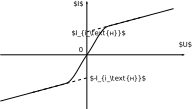
\includegraphics[width=0.5\textwidth]{Chapter_5/v5_11}
	\caption{Вольт-амперная характеристика двойного зонда}
	\figmark{Double probe VAC}
\end{wrapfigure}

Графики типа рис.~\figref{Double probe VAC} проще всего обрабатывать следующим образом. Сначала находится $I_{i\text{н}}$ из пересечения асимптот
с осью $U=0$. Затем, по наклону асимптот, находится величина $A$. После этого из \eqref{5.42} нетрудно определить $T_e$.
Дифференцируя эту формулу по $U$ в точке $U=0$ и принимая во внимание, что при малых аргументах $\th\alpha\approx\alpha$,
а при малых наклонах кривой насыщения $A\to 0$, найдём
\begin{equation}
	\eqmark{5.43}
	kT_e=\frac12\frac{eI_{i\text{н}}}{\left.\frac{dI}{dU}\right|_{U=0}}.
\end{equation}

Концентрацию плазмы $n$ можно найти из формулы \eqref{5.31}. Как это уже ясно из сказанного, двойные зонды удобно применять
для измерения электронной температуры и концентрации электронов в плазме.